\documentclass[a4paper]{article}

\usepackage[english]{babel}
\usepackage[latin1]{inputenc}
\usepackage{amssymb}
\usepackage{framed}
\usepackage{graphicx}
\usepackage{subcaption}
\usepackage{float}

\setlength{\parindent}{0pt}
\setlength{\parskip}{3ex}

\begin{document}

\begin{center}
  {\large Artificial Neural Networks and Deep Architectures, DD2437}\\
  \vspace{7mm}
  {\huge Short report on lab assignment 2\\[1ex]}
  {\Large Radial basis functions, competitive learning and self-organisation}\\
  \vspace{8mm}  
  {\Large Etienne Jodry, Frano Rajic, Ivan Stresec\\}
  \vspace{4mm}
  {\large September 20, 2020\\}
\end{center}

%\begin{framed}
%Please be aware of the constraints for this document. The main intention here is that you learn how to select and organise the most relevant information into a concise and coherent report. The upper limit for the number of pages is 6 with fonts and margins comparable to those in this template and no appendices are allowed. \\
%These short reports should be submitted to Canvas by the authors as a team before the lab presentation is made. To claim bonus points the authors should uploaded their short report a day before the bonus point deadline. The report can serve as a support for your lab presentation, though you may put emphasis on different aspects in your oral demonstration in the lab.
%Below you find some extra instructions in italics. Please remove them and use normal font for your text.
%\end{framed}

\section{Main objectives and scope of the assignment}

%\textit{List here a concise list of your major intended goals, what you planned to do and what you wanted to learn/what problems you were set to address or investigate, e.g.}\\
Our major goals in the assignment were  
\begin{itemize}
\item to analyze the behaviour of RBF networks with respects to different hyperparameters
\item to analyze the behaviour of RBF networks in respect to noisy data
\item to use and tune Self Organizing Maps unsupervised learning technique to find structure in data
\end{itemize}

%\textit{Then you can write two or three sentences about the scope, limitations and assumptions made for the lab assignment}\\

To experiment with RBF networks, we have used two function: the sine wave $sin(2x)$ and the $square(2x)$ function and tested many different parameters and methods as well as the impact of noise in the dataset. We also used competitive learning for clustering and determining the centres of RBFs and finally tested RBF networks on a 2-dimensional ballistical experiment. In the second part of the lab we tested SOMs in three different problems: ordering of animals, cyclic tour and clustering.

\section{Methods}

We have used Python 3.8 with some of its built-in libraries along with Matplotlib and NumPy libraries for all of our experiments. We also often used Google Sheets for result analysis and visualization.

%Here are the answers to some questions in the part "background". TODO

%When computing the weight matrix between the hidden and the output layer, one comes upon the system of equations shown in equation /ref{AE}. If N > n, the system is overdetermined so we cannot use Gaussian elimination directly to solve for w. In fact, in practice there is no exact solution to /ref{AE}.

%The lower bound for the number of training examples, N, is the number of hidden nodes, n. Having N<n tends to give bad overfitting results and should never be used. More data is needed. If the case that N=n, the equation /ref{AE} boild down to the square matrix PHI (times weight vector w to give vector f). For square matrices, an inverse can exist if and only if the matrix is not singular. For non singular matrices, there exists a inverse PHI-1 that can then be used to give a solution for w. That solution will give error equal zero. In the case a singular matrix is encountered, only a pseudoinverse can be used to determine the least squares solution for w. The pseudoinverse is, in fact, equal to the real inverse, if the inverse exists. If there is no inverse, then a pseudoinverse can be used to get the exact solution with lowest error.

%During training we use an error measure defined over the training examples. Note that it is not good to use this measure when evaluating the performance of the network. The measured train metric is biased towards the data that was seen in the training set, and therefore cannot give a useful and unbiased measure of the generalization performance for unseed data. The ability of having a unbiased and more reliable estimator of  the real generalization performance is exactly why train-test splits are used.

\section{Results and discussion - Part I: RBF networks and Competitive Learning}

%\begin{framed}
%\textit{Make effort to be \textbf{concise and to the point} in your story of what you have done, what you have observed and demonstrated, and in your responses to specific questions in the assignment. You should skip less important details and explanations. In addition, you are requested to add a \textbf{discussion} about your interpretations/predictions or other thoughts concerned with specific tasks in the assignment. This can boil down to just a few bullet points or a couple of sentences for each section of your results. \\ Overall, structure each Results section as you like. Analogously, feel free to group and combine answers to the questions, even between different experiments, e.g. with noise-free and noisy function approximation, if it makes your story easier to convey. \\
%\\Plan your sections and consider making combined figures with subplots rather than a set of separate figures. \textbf{Figures} have to condense information, e.g. there is no point showing a separate plot for generated data and then for a decision boundary, this information can be contained in a single plot. Always carefully describe the axes, legends and add meaningful captions. Keep in mind that figures serve as a support for your description of the key findings (it is like storytelling but in technical format and academic style. \\
%\\Similarly, use \textbf{tables} to group relevant results for easier communication but focus on key aspects, do not overdo it. All figures and tables attached in your report must be accompanied by captions and referred to in the text, e.g. $"$in Fig.X or Table Y one can see ....$"$. \\
%\\When you report quantities such as errors or other performance measures, round numbers to a reasonable number of decimal digits (usually 2 or 3 max). Apart from the estimated mean values, obtained as a result of averaging over multiple simulations, always include also \textbf{the second moment}, e.g. standard deviation (S.D.). The same applies to some selected plots where \textbf{error bars} would provide valuable information, especially where conclusive comparisons are drawn.} 
%\end{framed}

\subsection{Function approximation with RBF networks}

The centres of RBF units are equally distanced inside of our input space $[0, 2\pi]$, the distance obviously depending on the number of RBF units. The variance of each RBF unit is equal to the square root of the distance as this showed good results in preliminary testing, unless differently specified.

Firstly, we have tested the RBF networks' ability to predict the values of the $sin(2x)$ and the $square(2x)$ functions without any noise and using the least square method (LSM), as described in the assignment 3.1.

The prediction of the $sin(2x)$ function need at least 6, 10, and 12 RBF units for an MAE lower than 0.1, 0.01, and 0.001, respectively. The performance was somewhat worse for $square(2x)$ as expected due to the shape of the function which is hard for an RBF network to describe.

\begin{figure}[h!]
    \centering
    \begin{subfigure}{.5\textwidth}
      \centering
      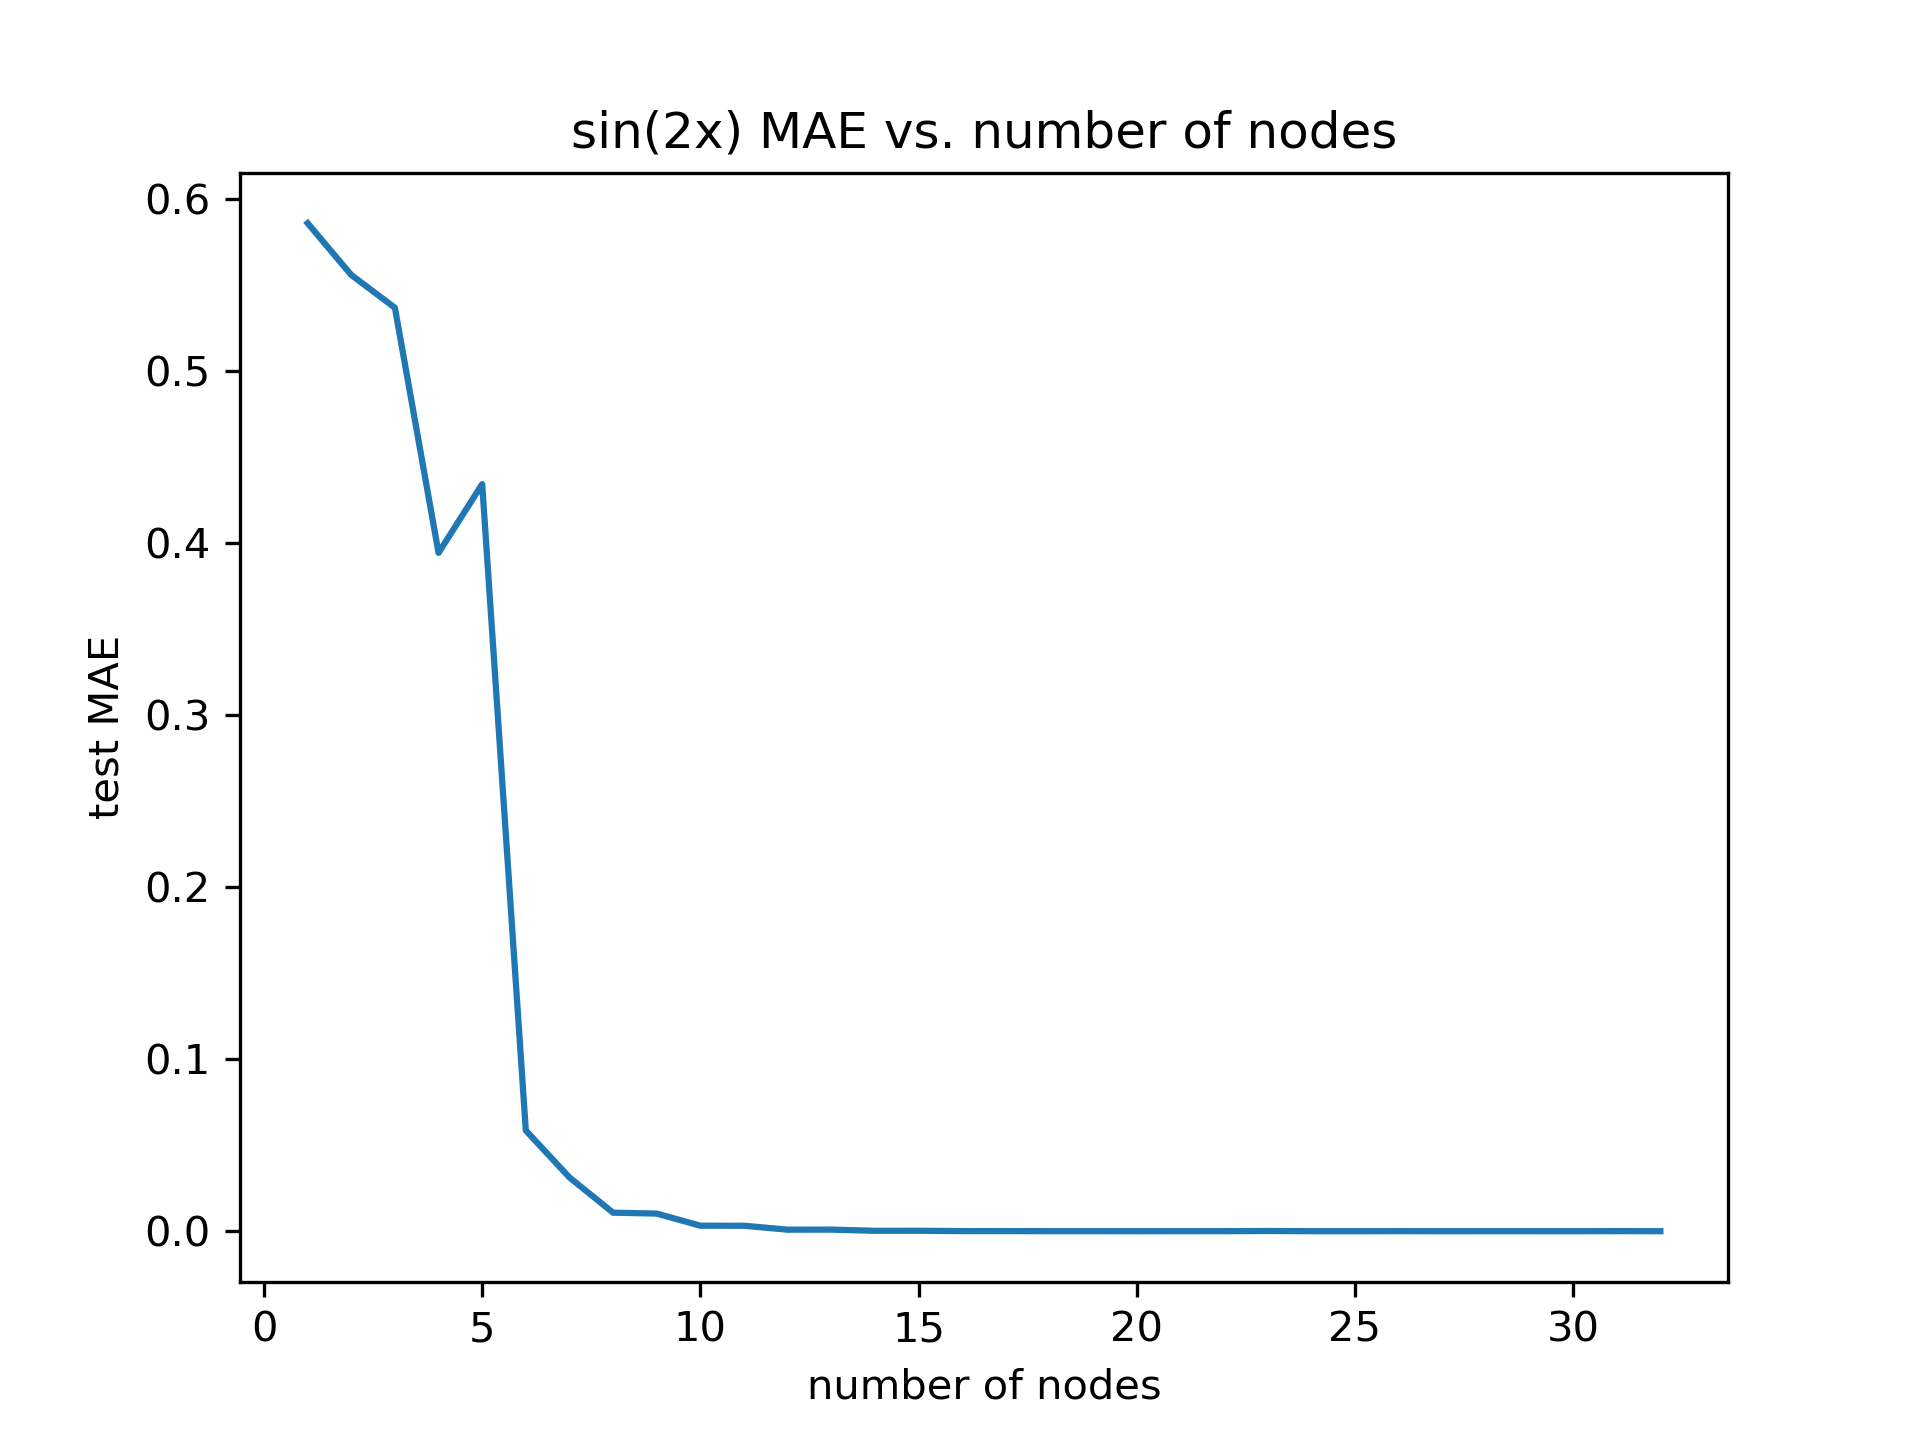
\includegraphics[width=1.0\linewidth]{img/3-1_sin2x.png}
      \caption{$sin(2x)$}
    \end{subfigure}%
    \begin{subfigure}{.5\textwidth}
      \centering
      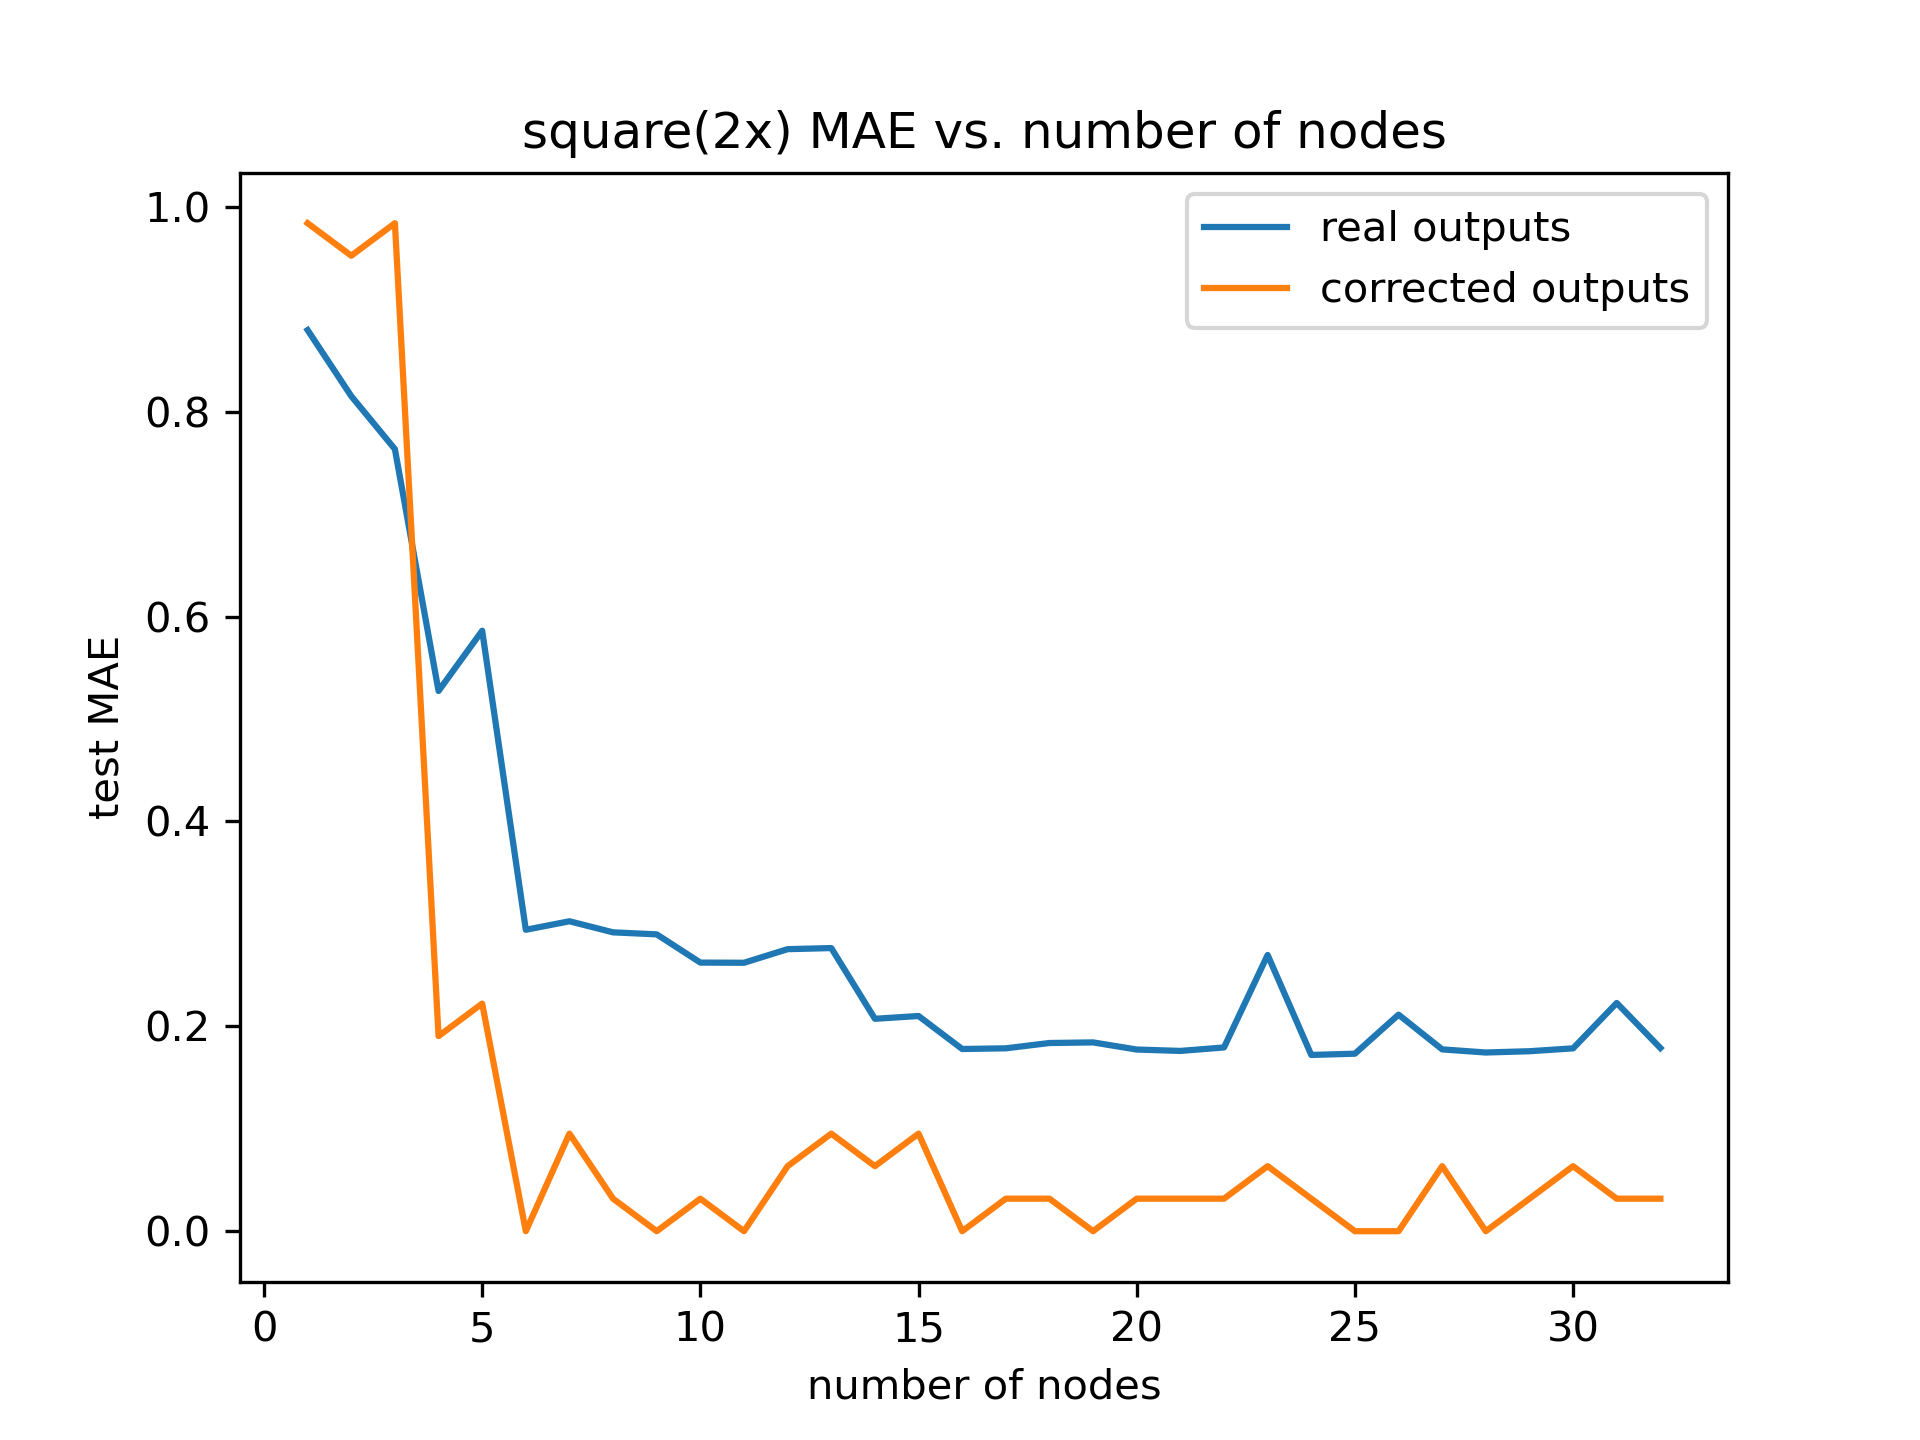
\includegraphics[width=1.0\linewidth]{img/3-1_square2x.png}
      \caption{$square(2x)$}
    \end{subfigure}
    \caption{Test MAE in relation to the number of nodes}
    \label{fig:3-1_performance}
\end{figure}

We can greatly improve the performance of the $square(2x)$ RBF network by using a sign ($sgn$) function. Using a sign function on the output of the network yielded an MAE of 0 with 6 RBF units. With a different distribution of RBF means we could perhaps reach an MAE of 0 with fewer nodes, e.g. placing 4 nodes in the middle of each half-period. Generally, this approach of mapping continuous values to discrete values can be used elsewhere; most obviously classification, but also regression with quantized outputs as we have seen here.

Secondly, we have added Gaussian noise with a standard deviation of 0.1 to our data and tested different RBF networks using the LSM as well as the online delta learning rule (DR). We have tested different learning rates, different RBF widths and different numbers of nodes for both the $sin(2x)$ and $square(2x)$ functions. For the delta rule we have used $25\%$ of the training set for early stopping validation. We have compared the test MAE of different configurations as this error demonstrates the generalisation capabilities best.

For the DR we have observed faster convergence with higher learning rates, but if the learning rate is too high the error would diverge. A higher number of nodes also slows down convergence.

When changing the widths of RBFs we observed that using too small or too large widths causes a decrease in performance. This can be intuitively explained by the RBFs covering too little or too much of the input space which renders them less capable of solving the problem (figure \ref{fig:3-2_rbf_width}).

\begin{figure}[h!]
    \centering
    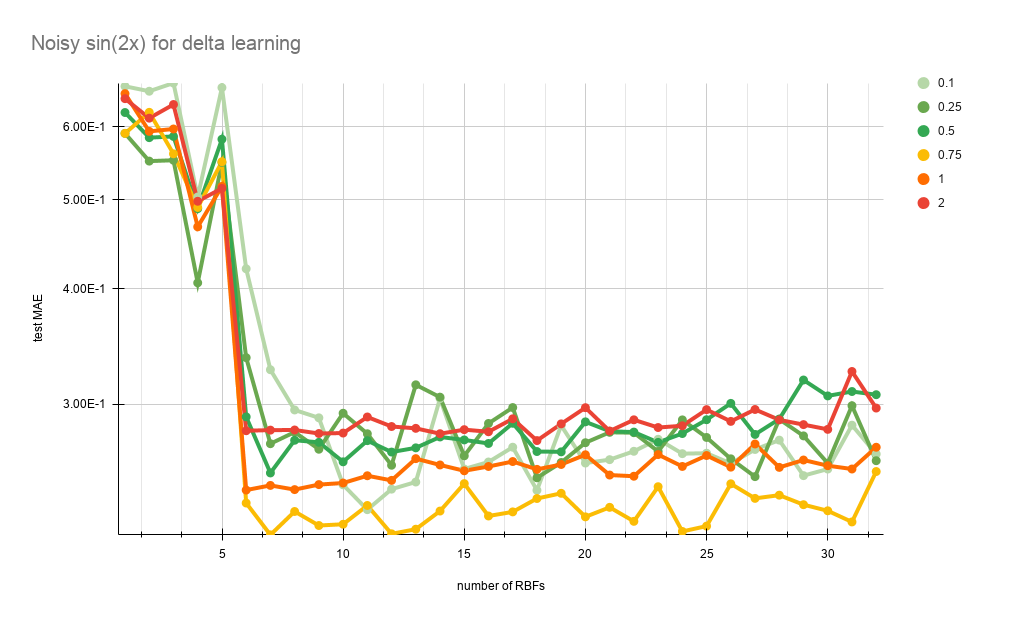
\includegraphics[width=0.8\linewidth]{img/3-2_widths.png}% :)
    \caption{The influence of RBFs' width on performance of the noisy sin(2x)}
    \label{fig:3-2_rbf_width}
\end{figure}

Picking random RBF centres worked worse than using our strategy of distributing the centers evenly across the input space. 

Generally, when using data without noise the LSM outperforms the DR, but when adding noise the DR outperforms the LSM. This is due to the fact that the LSM will find an optimal solution considering the training data, which leaves it exposed to overfitting on bad data, a problem which the DR (with early stopping) handles better.

We have compared our best performing RBF networks using the LSM with a two-layer perceptron with the same amount of nodes for the noisy $sin(2x)$ and $square(2x)$ and the RBF networks outperformed the perceptrons slightly in both problems. More general conclusions cannot be drawn.

\subsection{Competitive learning for RBF unit initialisation} % \\ \normalsize{\textit{(ca. 1 page)}}
%\textit{Please refer first to the results in the previous section, i.e. those obtained without any automated initialisation. Then in the next subsection focus on two-dimensional regression with RBF networks.}

\subsubsection{Waves}

We compared MAE performance with the previously used manual initialization for RBF centres versus automated initialisation using KMeans clustering algorithm. The tests were performed on the noisy and noiseless sine(2x) dataset used before. Manual LSM performed best on noiseless dataset, but automated initialization showed much better results than using manual delta. On the noisy dataset, the automated version was not better and not much worse than the manual initialization approach. The results are summed up in figure \ref{fig:3-3_sine_moj}. We did not monitor and compare convergence behaviour.

We noticed that dead units occurred when KMEans algorithm used random points to initialize centres. Using a random selection of train datapoints to initialize the centres made the KMeans algorithm never have dead units.

\begin{figure}[h!]
    \centering
    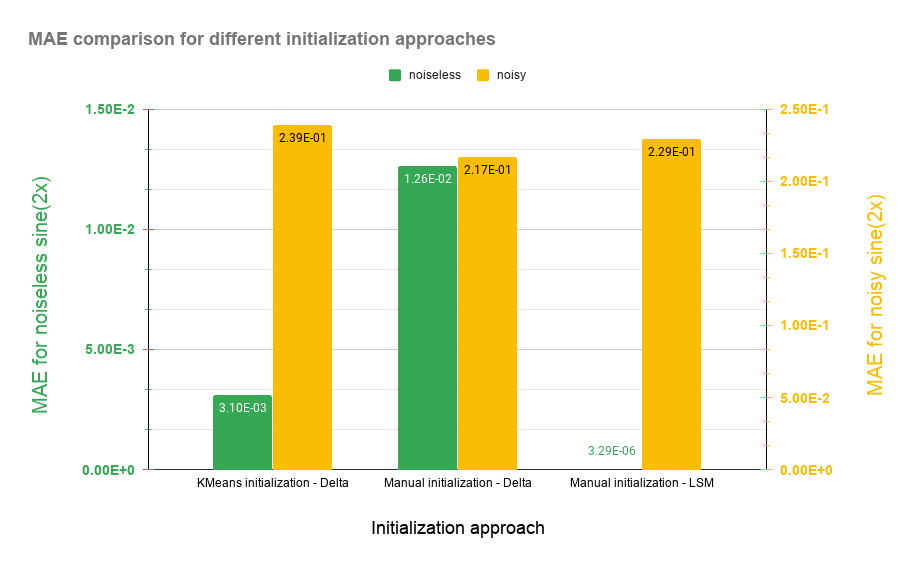
\includegraphics[width=0.8\linewidth]{img/3-3_sine_moj_3.png}
    \caption{MAE comparison for different initialization approaches}
    \label{fig:3-3_sine_moj}
\end{figure}

\subsubsection{Ballistical experiments dataset}

We used the automatically initialized RBFs for two-dimensional regression on the ballistical experiments dataset, which is very noisy itself. The datasets maps (distance, height) pairs to (angle, velocity). KMeans CL clustering was used to initialize RBF centres. Train and test sets were separated. Both had 100 data points. For the needs of early stopping, train set was further divided into two subsets. Different KMeans initialization configurations and RBF learning rates were tested. The network managed to learn the mapping with best MAE value going down to 0.00529 for learning rate of 0.25 and 30 RBF nodes. The resulting and expected functions as well as colored clusters and the positions of RBF centres are shown in figure \ref{fig:3-3_ballistic}. 

\begin{figure}[h!]
    \centering
    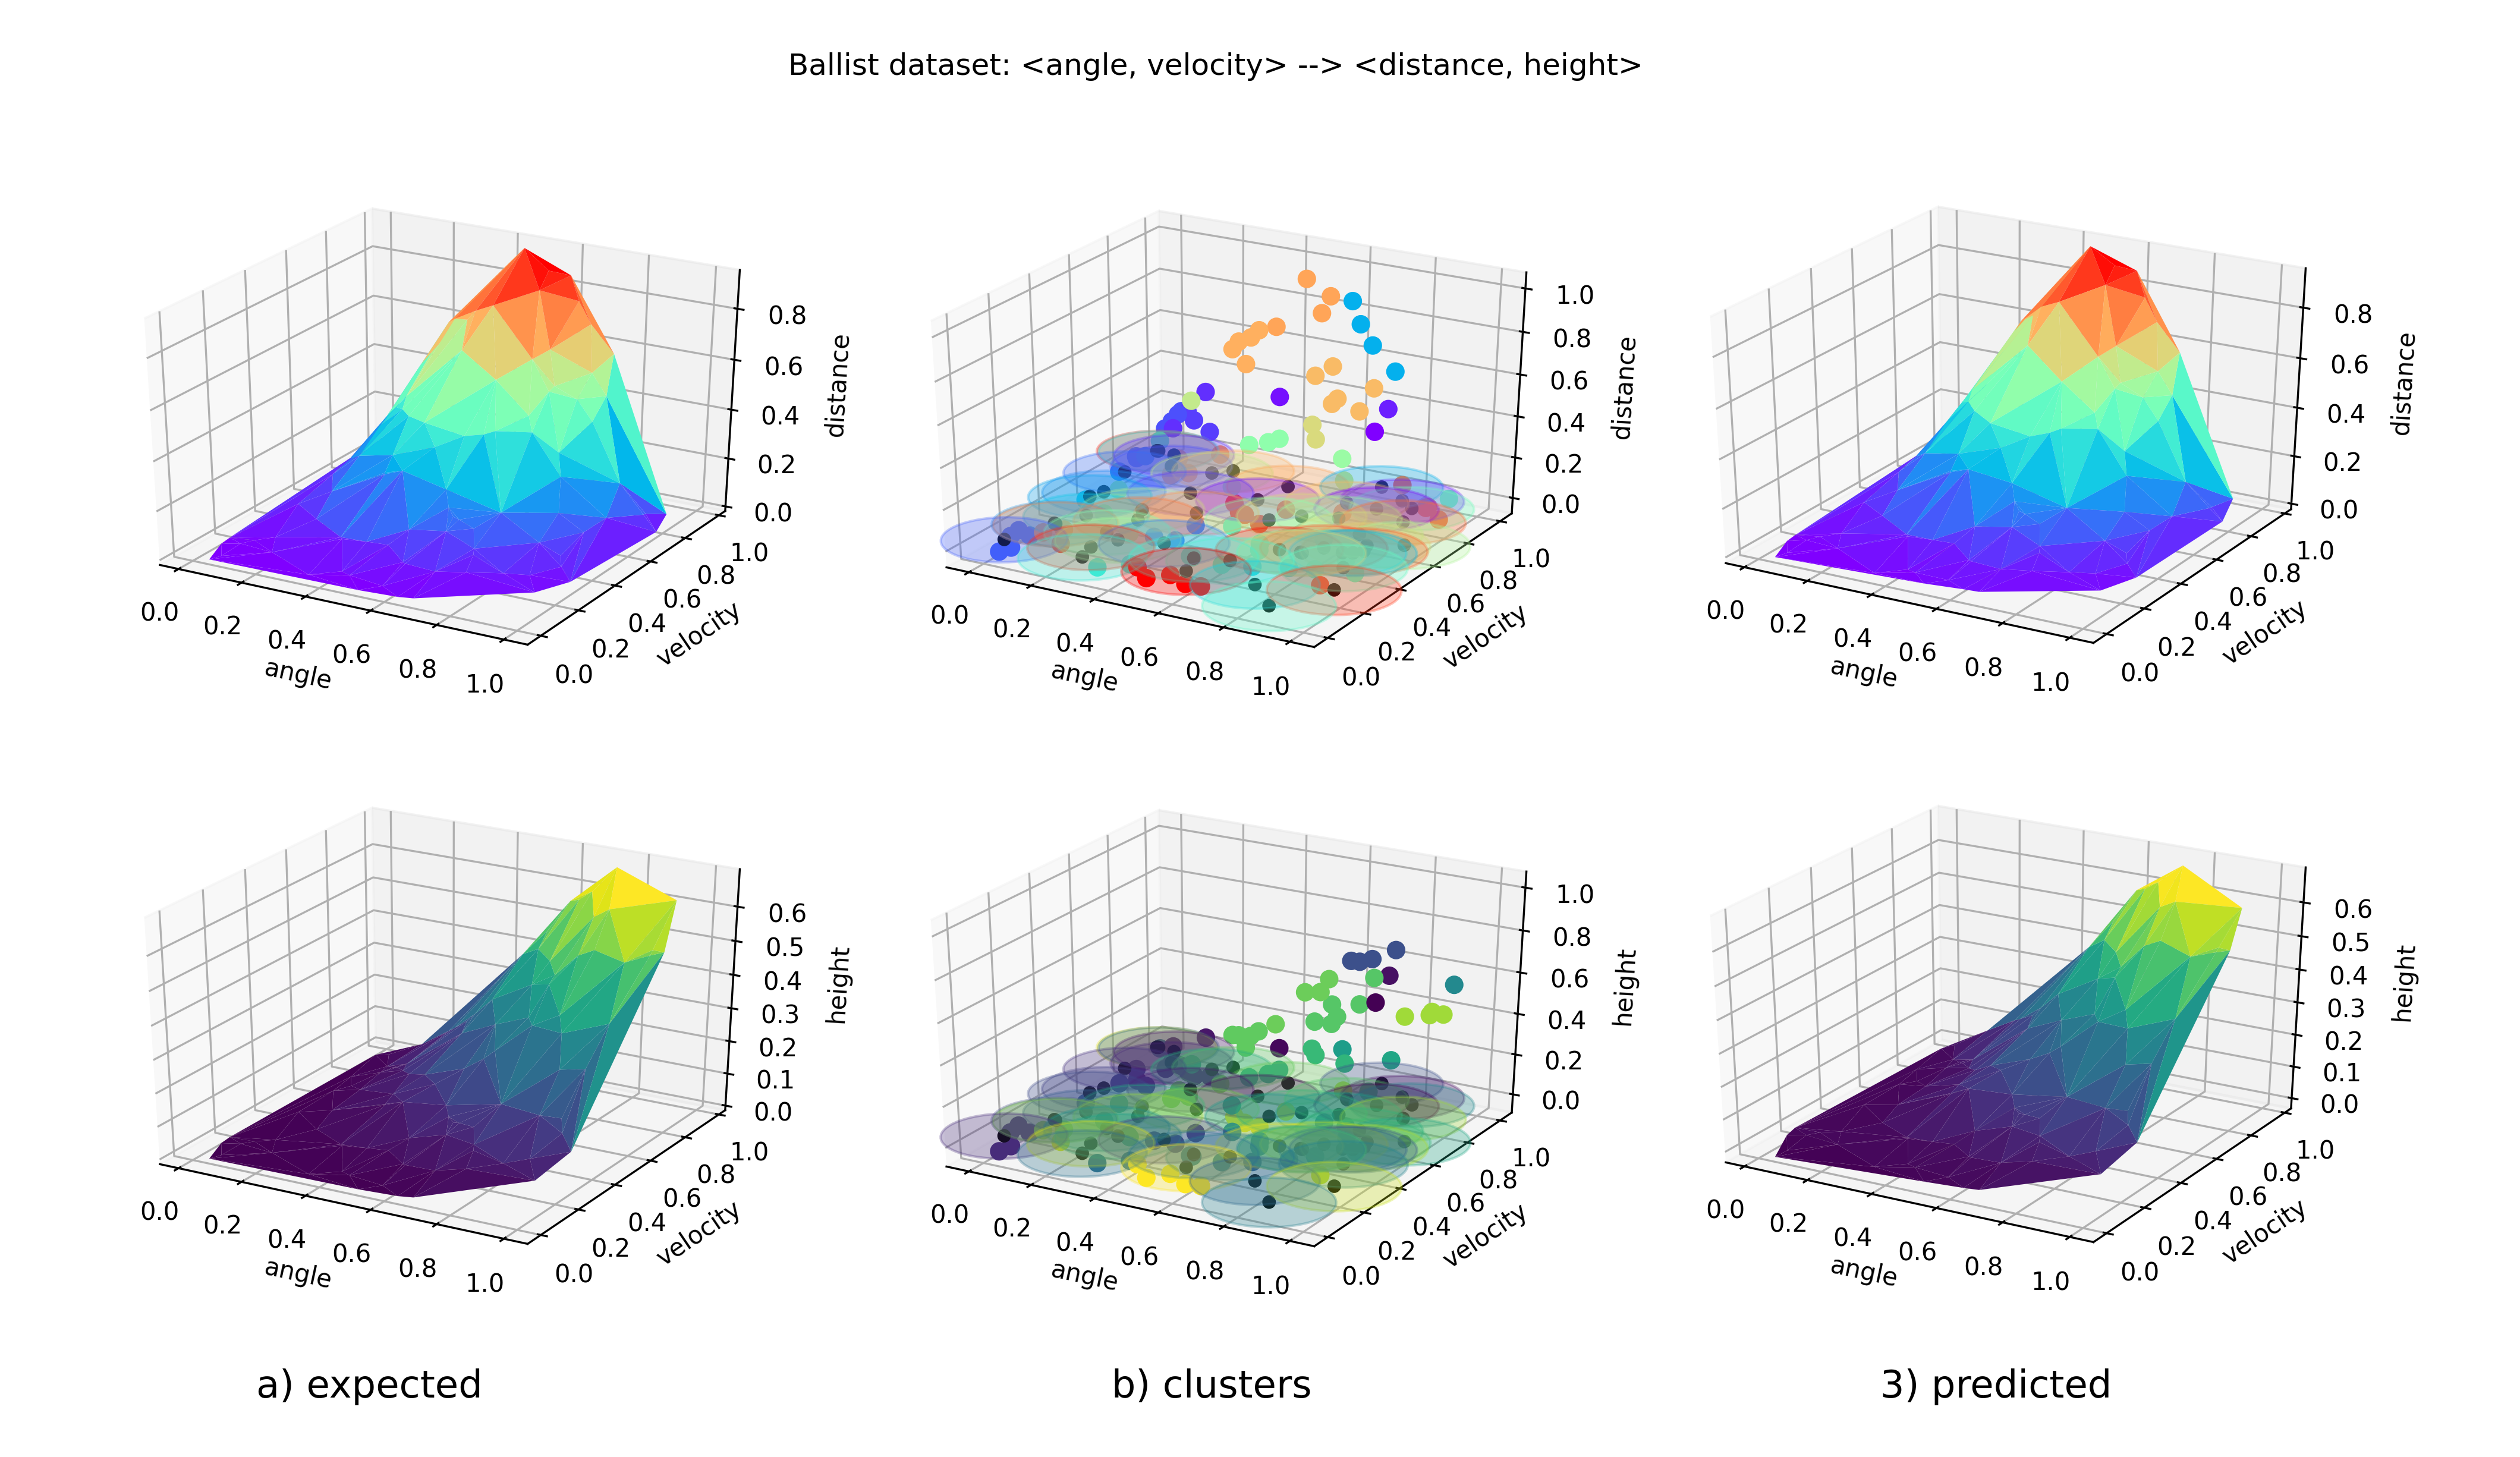
\includegraphics[width=\linewidth]{img/3-3_ballist.png}
    \caption{Results on ballistical experiments dataset. Left - expected formula. Middle - visualisation of RBF centres and corresponding clusters. Right - predicted function.}
    \label{fig:3-3_ballistic}
\end{figure}

\section{Results and discussion - Part II: Self-organising maps}

\subsection{Topological ordering of animal species}
Here is the output of the training with $100$ nodes, $\eta = 0.2$ and a neighborhood sequence that follows the harmonic series multiplied by $50$ in the beginning and ends with $2, 1$ and $0$.
\begin{figure}[H]
     \centering
\begin{verbatim}
('bat', 1), ('elephant', 4), ('horse', 7), ('pig', 10), ('giraffe', 12), 
('camel', 14), (antelope', 17), ('kangaroo', 20), ('rabbit', 22), ('rat', 25),
('cat', 27), ('lion', 29), ('ape', 32), ('skunk', 35), ('hyena', 38),
('dog', 40), ('bear', 44), ('walrus', 48), ('crocodile', 52),
(sea turtle', 55), ('frog', 59), ('penguin', 62), ('ostrich', 65),
('duck', 68), ('pelican', 71), ('spider', 77), ('housefly', 82), (mosquito', 85),
('butterfly', 88), ('beetle', 93), ('grasshopper', 95), ('dragonfly', 98), 
\end{verbatim}
\centering
\caption{SOM for animal species ordering: Input name vs output index}
    \label{fig:my_label}
\end{figure}

We can observe a natural organization of the data in terms of the neighborhoods: 
\begin{itemize}
    \item From 1 to 48: Mammals;  From 62 to 71 Birds;
    \item From  52 to to 71 Chordates; From 77 to 98 Insects\footnote{We include spider as an insect even though it is an arachnid, no offense intended to any biologists reading this :)}
    \item Cat \& Lion; Hyena \& Dog; Kangaroo \& Rabbit are neighbors
    \item \ldots
\end{itemize}

\subsection{Cyclic tour}
On the left of figure \ref{fig:SOM_TSP} we see a SOM trained with $10$ nodes (one for each city), $\eta = 0.65$, $20$ epochs, and the majority of the neighborhood sequence equal to zero (individual updates), so a nice specialization can happen.

We show the vectors as points in the input space and we can see they constitute a solution to traveling salesman problem if we connect them. The learning rate has to be a bit higher this time as otherwise we observe that the vectors may stay "stuck" between cities and not converge, which can be seen on the right side of figure \ref{fig:SOM_TSP}: $\eta = 0.225$.

\begin{figure}[h!]
    \centering
    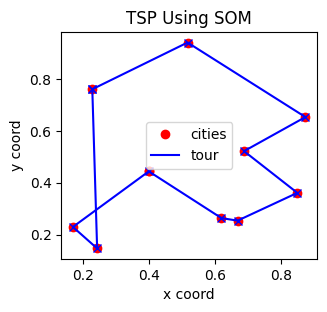
\includegraphics[width=.33\linewidth]{img/SOM_tsp.png}
    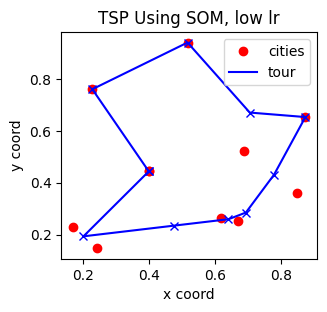
\includegraphics[width=.33\linewidth]{img/SOM_tsp_low_lr.png}
    \caption{Cities: SOM vectors shown in the input space}
    \label{fig:SOM_TSP}
\end{figure}

\subsection{Clustering with SOM}
This part was a little trickier as we had to train the model separately with the result of the vote and one of the 3 metrics we hoped to do clustering on ($\in$\{sex, party, district\}), and finally build a map as shown in figure \ref{fig:SOM_MP}, associating each point to said metric.

\begin{figure}[h!]
    \centering
    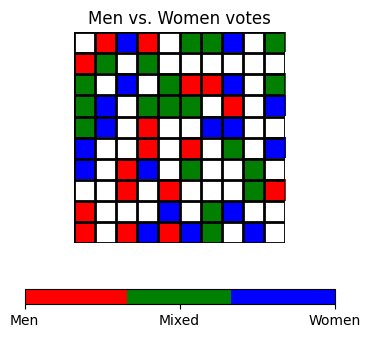
\includegraphics[width=.4\linewidth]{img/SOM_mp_sex.png}
    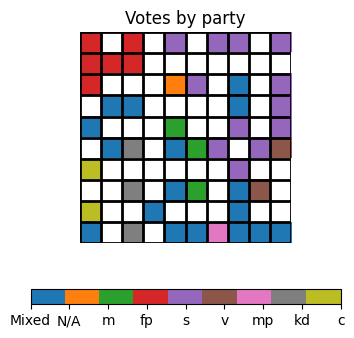
\includegraphics[width=.4\linewidth]{img/SOM_mp_party.png}
    \caption{MP Votes: SOM $10\times10$ Colormap in respect to sex or party}
    \label{fig:SOM_MP}
\end{figure}

Even when with severe varying of the neighborhood sequence and the learning rate, we got a lot of results as the one shown in figure \ref{fig:SOM_MP}: numerous mixed squares and no structure on gendered ones. Given these results, one could claim that in a country such as Sweden there is actually no gender difference in respect to votes in the parliament and do so with evidence.

On the other hand, we managed to get nice party clusters that even reflect the sizes of each party (Social Democrat party which was in majority during 2004-2005). There are also geometric intuitions that are related to the actual structure of parliament\footnote{Aylot, Nicholas (2015) The Party System} that can be derived from the graphic as clusters of the social democrat (S) party and the left party (V) are close - they had an agreement during this mandate. The moderate (M) cluster is in the middle as well.

\begin{figure}[h!]
    \centering
    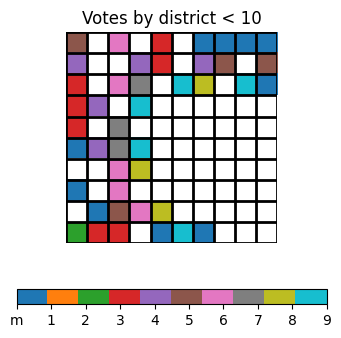
\includegraphics[width=.25\linewidth]{img/SOM_mp_d10.png}
    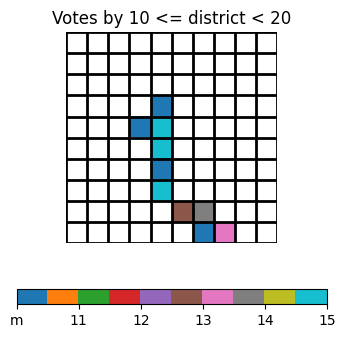
\includegraphics[width=.25\linewidth]{img/SOM_mp_d20.png}
    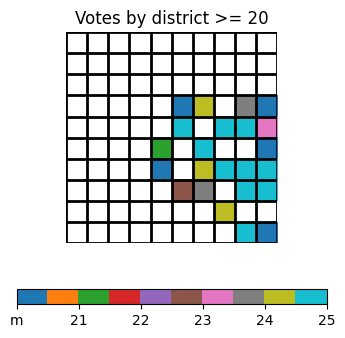
\includegraphics[width=.25\linewidth]{img/SOM_mp_d30.png}
    \caption{MP Votes: SOM in respect to Districts split in 3 plots}
    \label{fig:SOM_MP_D}
\end{figure}

For figure \ref{fig:SOM_MP_D} we split district plots in 3 for readability reasons. Since there is so many districts is is hard to derive conclusions but we can see general clustering tendencies, particularly when comparing districts from 0 to 9 vs. districts from 20 to 25.



\section{Final remarks} %  \normalsize{\textit{(max 0.5 page)}}
% \textit{Please share your final reflections on the lab, its content and your own learning. Which parts of the lab assignment did you find confusing or not necessarily helping in understanding important concepts and which parts you have found interesting and relevant to your learning experience? \\
% Here you can also formulate your opinion, interpretation or speculation about some of the simulation outcomes. Please add any follow-up questions that you might have regarding the lab tasks and the results you have produced.}
The part about unsupervised learning was a bit confusing as there is no real metric to compare results. We produced a lot of graphs and kept the models that resulted in the most visually satisfying plots, but it was definitely not convenient for hyper-parameter searching. The neighborhood sequence requires a lot of tuning as well, which could be seen as tuning several hyper-parameters.
For the last question of the assignment concerning the Swedish parliament, even if the clustering did work well, it was not easy to derive conclusions without knowing much about Swedish political system. This also made it interesting.

\end{document}
